
\subsection{Vista de casos de uso}

A partir de los casos de uso descritos en la sección~\ref{sec:casos-uso} y 
en la figura~\ref{fig:uml:casos-uso}, se refinaron para extaer una serie 
de casos de uso:

\begin{itemize}
 \item Parametrizar el sistema
 \item Publicar
 \item Enriquecer los datos
 \item Consular los archivos generados
 \item Consultar la información extra generada
\end{itemize}

Se pasará por tanto a describir cada caso de uso en profundidad mediante diagramas
actividas.

\subsubsection{Parametrizar el sistema}

Este caso de uso representa la labor que el usuario administrador debe realizar 
para configurar correctamente el sistema. En la figura~\ref{fig:uml:parametrizar-sistema}
se puede ver el diagrama de actividad de este caso de uso.

\begin{figure}[ht]
 	\centering
	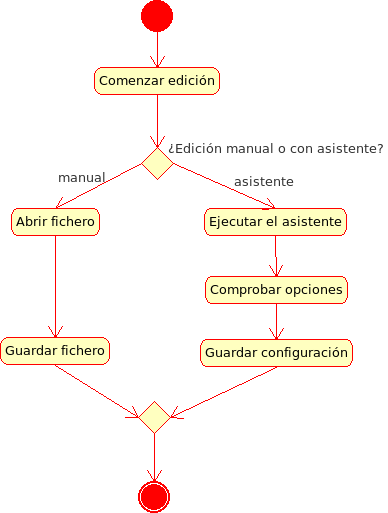
\includegraphics[width=8cm]{images/uml/casos-uso/parametrizar-sistema.png}
	\caption{Diagrama de actividad para el caso de uso «parametrizar el sistema»}
	\label{fig:uml:parametrizar-sistema}
\end{figure}

\subsubsection{Publicar}

Representa la acción de publicación propiamente dicha. El proceso es un proceso por 
lotes que a partir de una configuración genera una serie de ficheros RDF. Internamente
se descompone en varias actividades menores tal y como describe la 
figura~\ref{fig:uml:publicar}.

\begin{enumerate}
 \item \emph{Parsear} el mailbox
 \item Revisar la consistencia de todas las relaciones entre los distintos mensajes
 \item Enriquecer la información
 \item Exportar cada uno de estos mensajes en RDF
 \item Exportar los suscriptores en RDF
 \item Exportar los suscriptores en KML si fuese requerido
 \item Exportar todos los indices
\end{enumerate}

\begin{figure}[ht]
 	\centering
	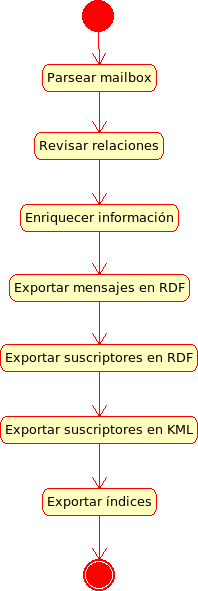
\includegraphics[width=4cm]{images/uml/casos-uso/publicar.png}
	\caption{Diagrama de actividad para el caso de uso «publicar»}
	\label{fig:uml:publicar}
\end{figure}

\subsubsection{Enriquecer los datos}

Representa la interacción del sistema con otras bases del conocimiento externas, 
principalmente los FOAF de los suscriptores a la lista de correo, para enriquecer 
la información en determinados aspectos.

Para cada suscriptor debe repetirse las tareas representadas en la 
figura~\ref{fig:uml:enriquecer}:

\begin{enumerate}
  \item Buscar su FOAF
  \item Si lo tiene:
	\begin{enumerate}
	  \item	Enlazar al suscriptor con su FOAF
	  \item Consultar sus coordenadas geográficas
	  \item Consultar su foto
	\end{enumerate}
  \item Si no lo tiene continuar con el siguiente suscriptor
\end{enumerate}

\begin{figure}[ht]
 	\centering
	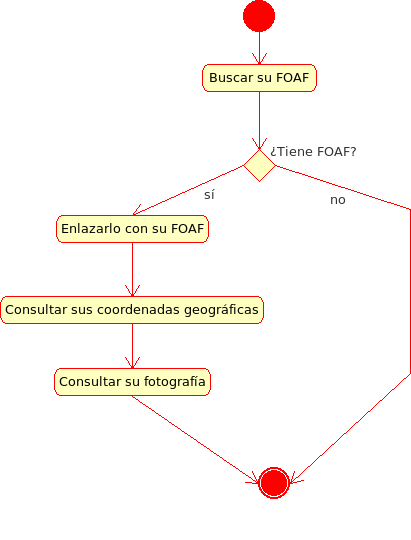
\includegraphics[width=8cm]{images/uml/casos-uso/enriquecer.png}
	\caption{Diagrama de actividad para el caso de uso «enriquecer datos»}
	\label{fig:uml:enriquecer}
\end{figure}

\subsubsection{Consular los archivos generados}

Representa la interacción del usuario con los datos generados. Desde una 
simple consulta manual a los ficheros RDF generados, hasta realizar 
consultas de una forma más sofisticada.

Con la información obtenida se repetirá siempre el mismo flujo descrito en
la figura~\ref{fig:uml:consultar}

\begin{enumerate}
 \item consultar
 \item leer
 \item comprender
 \item y/o desechar
\end{enumerate}

\begin{figure}[ht]
 	\centering
	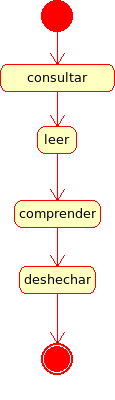
\includegraphics[width=3cm]{images/uml/casos-uso/consultar.png}
	\caption{Diagrama de actividad para el caso de uso «consultar»}
	\label{fig:uml:consultar}
\end{figure}

\subsubsection{Consultar la información extra generada}

Este caso de uso representa la consulta por parte del usuario de la 
información extra generada, por el ejemplo los suscriptores en formato 
KML. Las actividades son las que se pueden ver en la 
figura~\ref{fig:uml:consultar-extra}.

\begin{figure}[ht]
 	\centering
	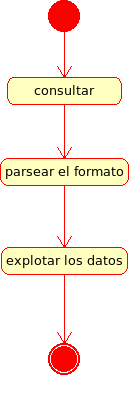
\includegraphics[width=3cm]{images/uml/casos-uso/consultar-extra.png}
	\caption{Diagrama de actividad para el caso de uso «consultar información extra»}
	\label{fig:uml:consultar-extra}
\end{figure}

